%Template generated by Ben Manning
%Purdue University
%btmannin@purdue.edu
%Last modified: 7/7/2021


\documentclass[notitlepage, 12pt]{report}  %The document class will setup a lot of basic formatting.  Report class will start with justifying paragraphs setup your different types of sections.

%Different packages allow you to add more functions that will make your time in LaTeX easier.
\usepackage{amsmath}
\usepackage{graphicx}
\usepackage{caption}
\usepackage{url}
\usepackage{circuitikz} % circuit drawer

%\usepackage{biblatex} %Imports biblatex package
\usepackage[style=numeric]{biblatex}
\addbibresource{bib.bib}

\usepackage[top=2cm, bottom=2cm, left=2cm, right=2cm]{geometry}

\title{Experiment 2 Report}

\graphicspath{{./images}}

\begin{document}
%Everything needs to begin and end.  


\begin{center}
\large \textbf{Experiment 2 Report} \\ %\large and \small can help make text sizes vary throughout your document.
%\textbf will bold the text that is in the curly brackets
\small 
Andrew Lykken\\
Anna Kishnani\\
26 January 2023\\
Section 004 (Abraham Yakisan)\\
%\rule{500pt}{.1pt} 

\end{center}

% space between title and abstract
\vspace{4in}


\begin{abstract}
This experiment focuses on driving a 12V motor with a RFD3055LE power transistor, and creating a control circuit to 
determine motor speed from a control voltage. We created a test circuit to determine core properties of the RFD3055LE 
power transistor, and used those properties to create a 555 timer circuit with a potentimeter to determine control 
voltage and create a model for motor speed from control voltage.  
\end{abstract}

\newpage

\section*{Task 1} %Each task has a section including (but not limited to) Objective, 
% Procedure, Results / Calculations, Conclusions


\subsection*{Objective}
\indent\indent The objective of this task is to experiment with the RFD3055LE power MOSFET to determine some 
of its core characteristics.

\subsection*{Procedure}
\indent\indent \textbf{Step 1-2}\\
The circuit below was constructed:

\begin{center}
    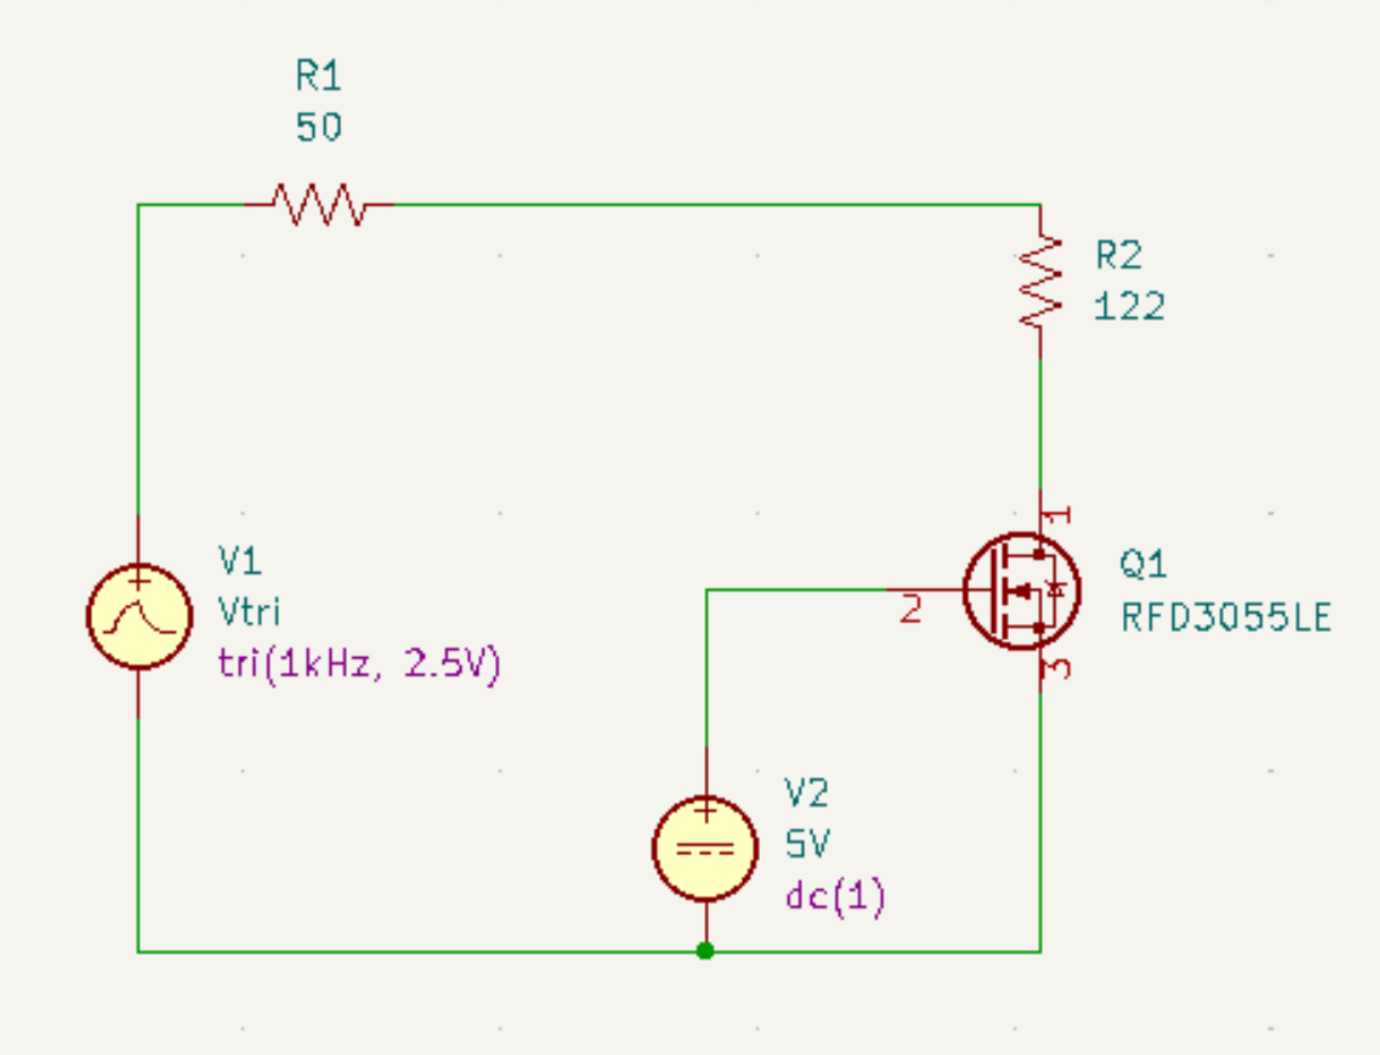
\includegraphics[scale=0.2]{task1.png}
\end{center}

and $R_{sense}$ was selected such that the maximum short circuit current of the circuit would be 30 mA. \\

\textbf{Step 3-4} \\
Using the oscilloscope, 4 curves were plotted in XY mode: One in the cutoff region, one in the linear region, and two in saturation. 
Labelled $v_{GS}$ for each curve. \\

\textbf{Step 5}\\
We estimated the power consumed by the transistor at each curve from \textbf{Step 3} by measuring the power at the largest
$v_{DS}$ value.\\

\textbf{Step 6-7}\\
We set $V_{gs}$ to be 5V and capture an oscilloscope screenshot, and estimated $R_{DS, on}$ using this. 
We compared the calculated $R_{DS, on}$ with that of the RFD3055LE datasheet. \\

\newpage

\subsection*{Results / Calculations}
\indent\indent \textbf{Step 3-4}\\
The following is a plot of the RFD3055LE power transistor in the cutoff region.\\

\begin{center}
    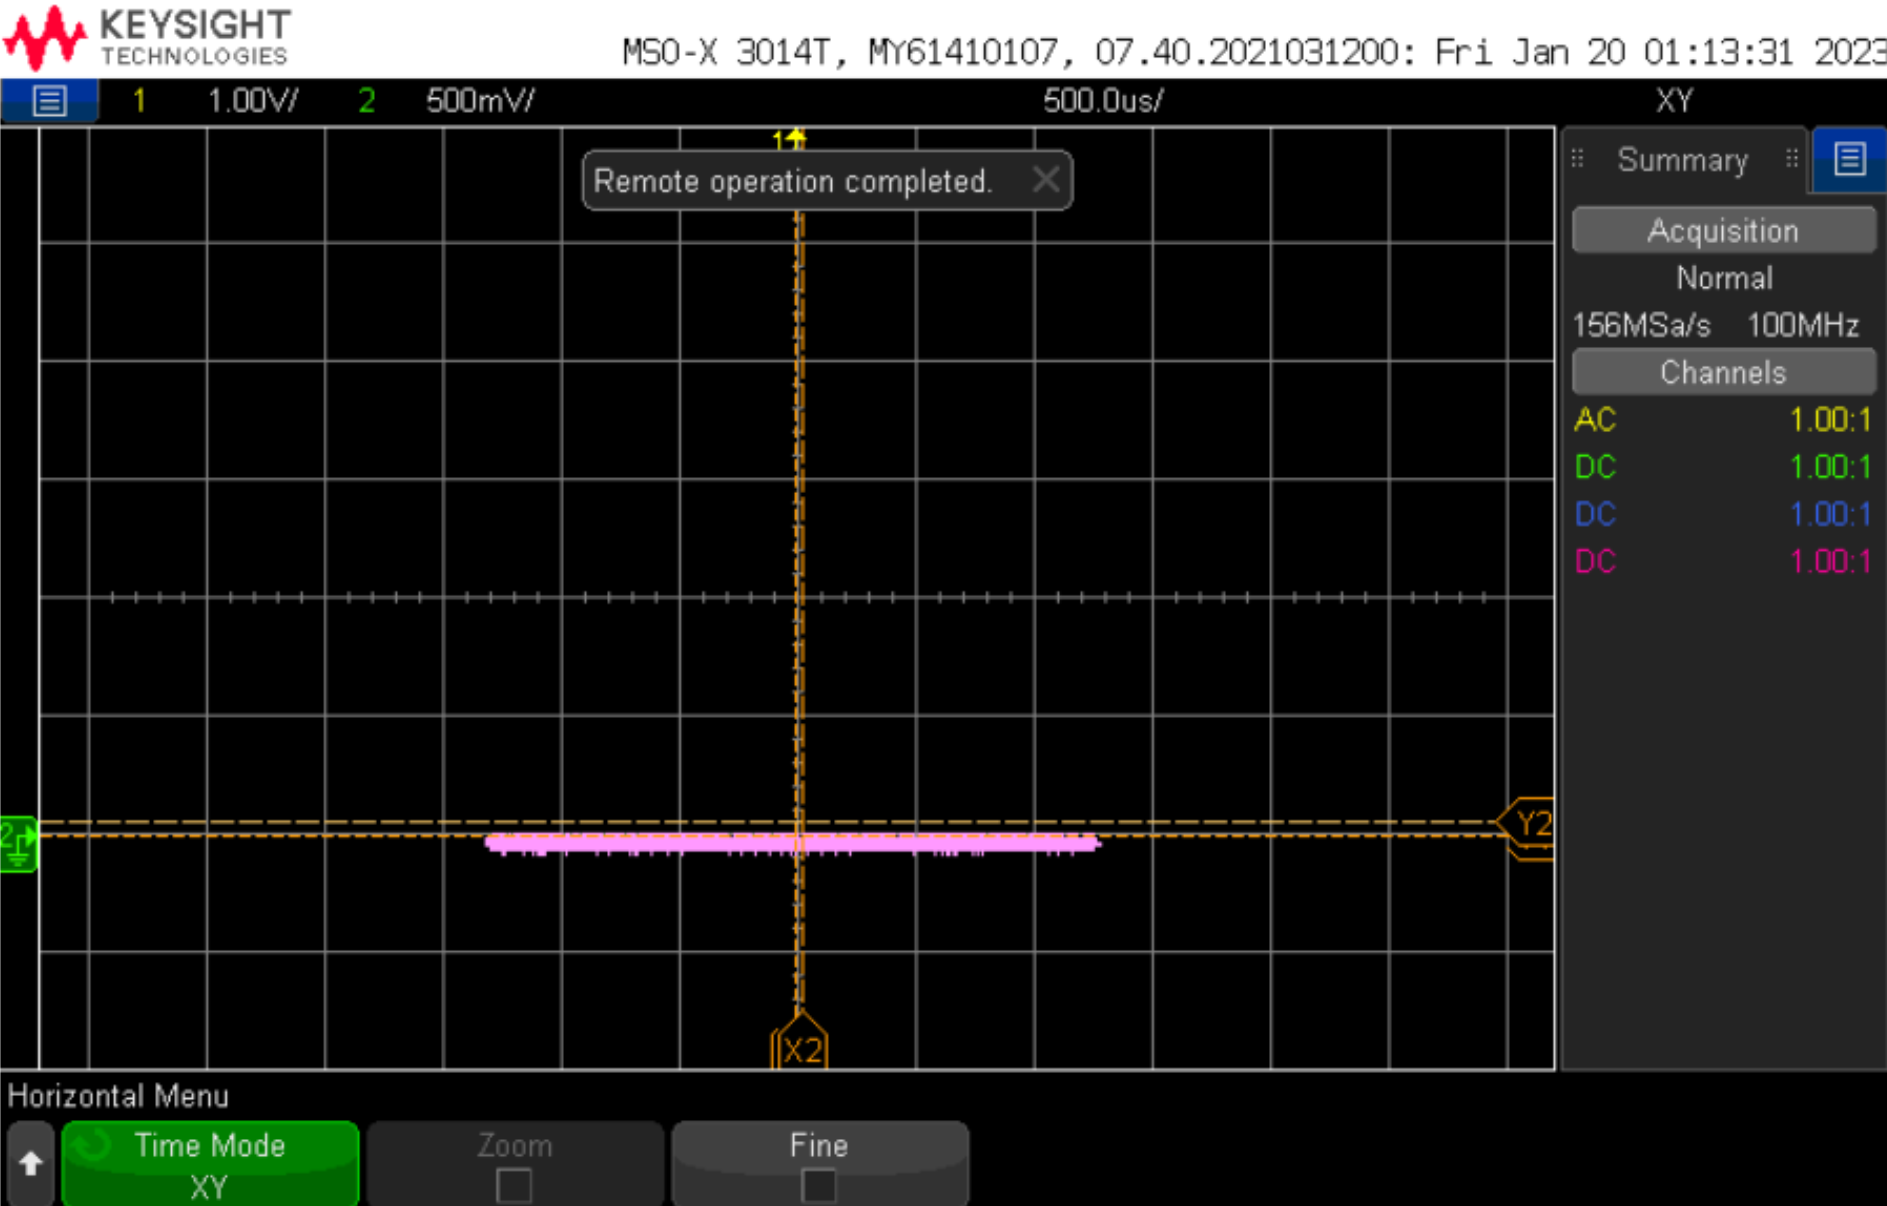
\includegraphics[scale=0.2]{cutoff.png}
\end{center}

\begin{center}
    $v_{GS}$ = 1.79V \\
\end{center}

The following are two plots of the RFD3055LE power transistor in the saturation region.\\

\begin{center}
    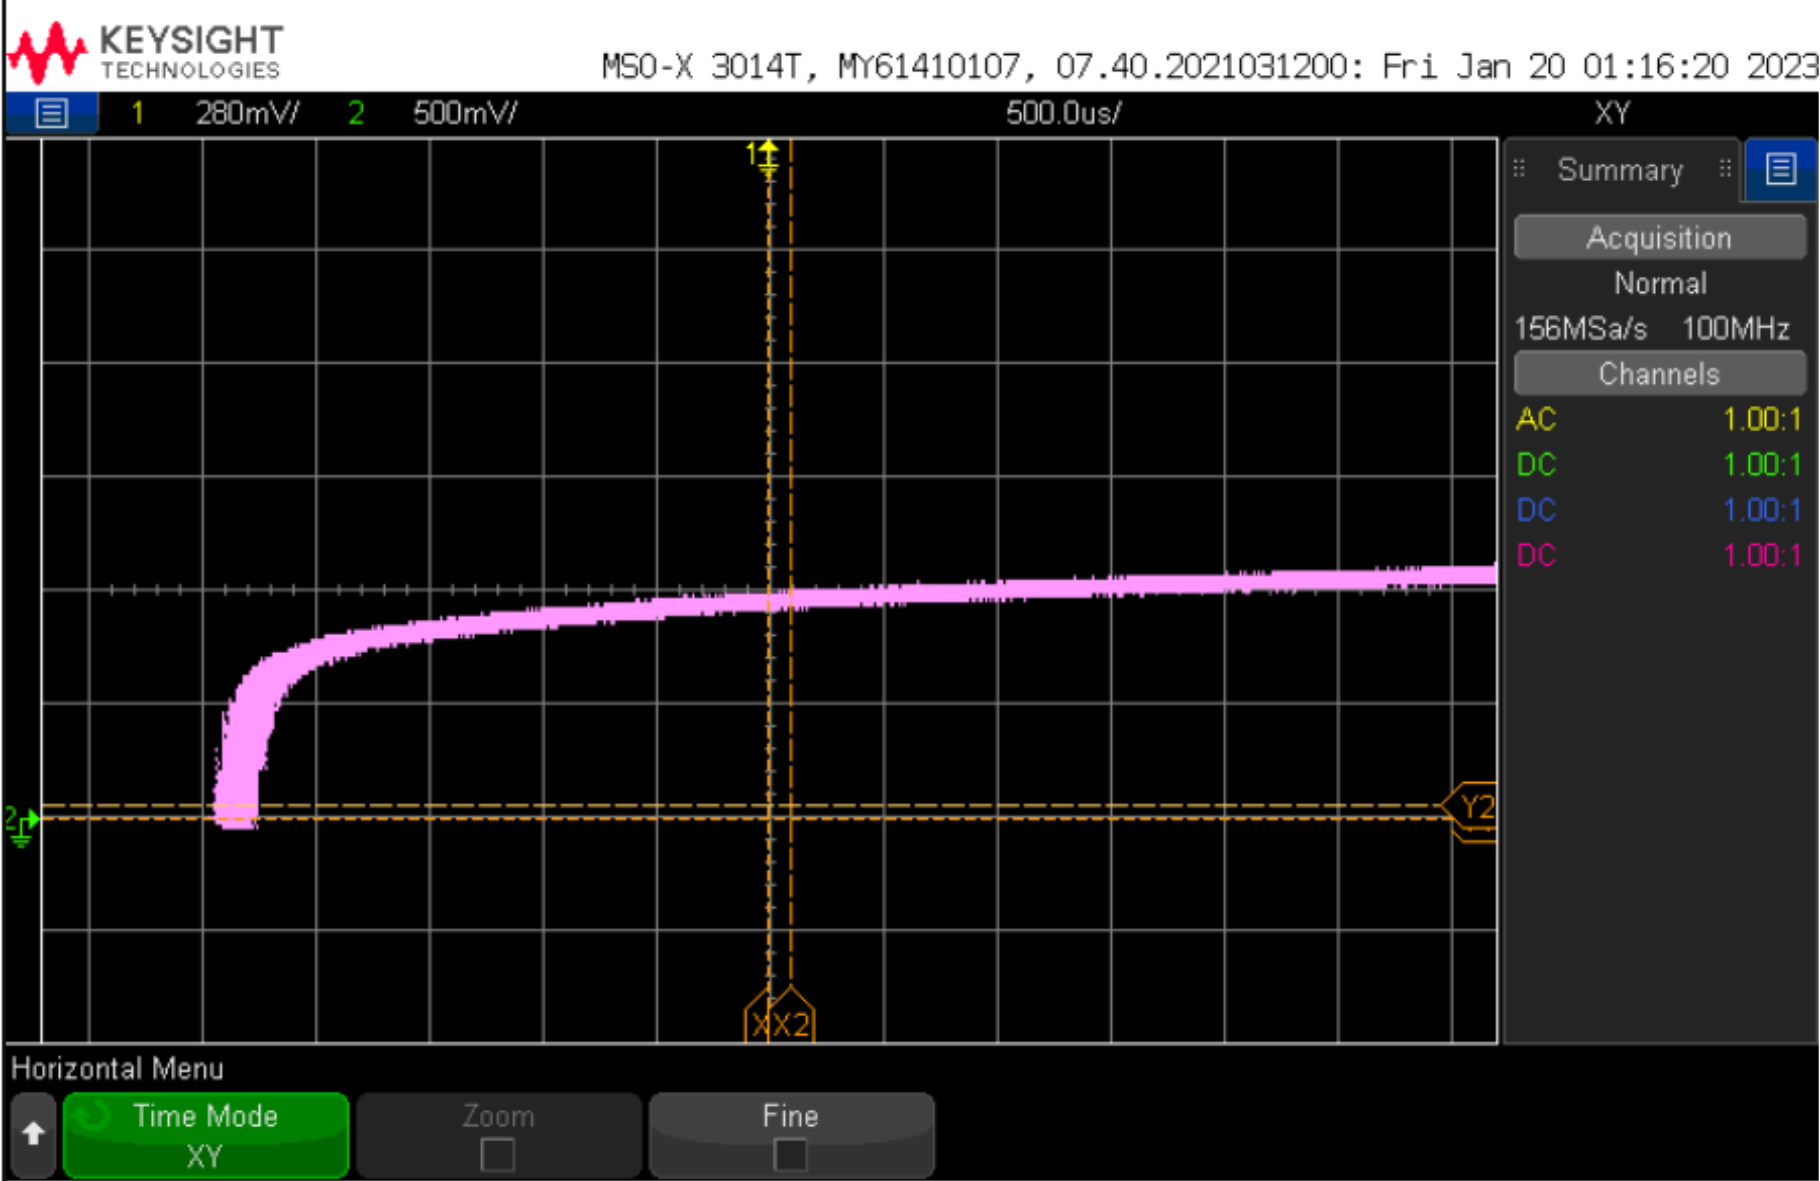
\includegraphics[scale=0.2]{sat1.png}
\end{center}

\begin{center}
$v_{GS}$ = 2.09V \\
\end{center}

\begin{center}
    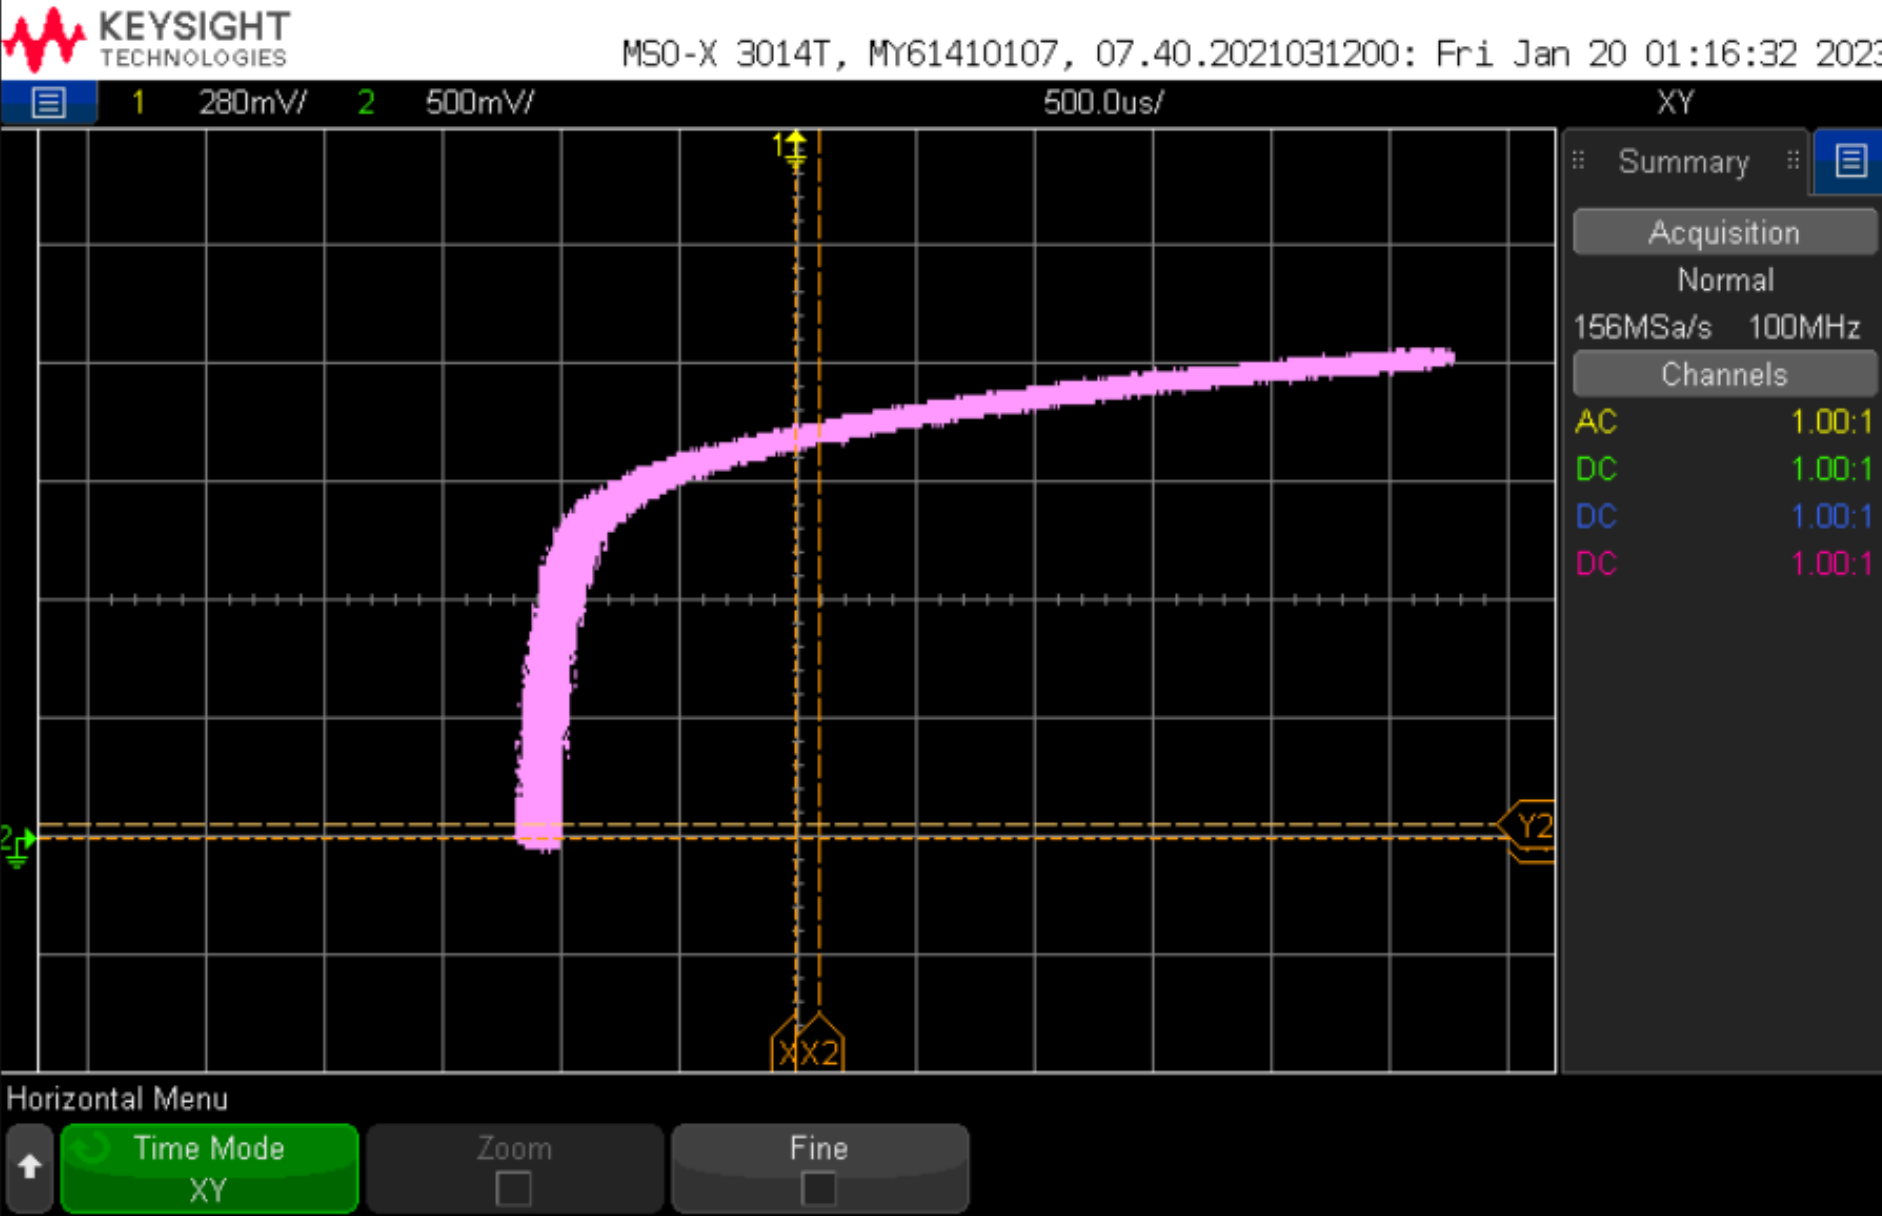
\includegraphics[scale=0.2]{sat2.png}
\end{center}

\begin{center}
$v_{GS}$ = 2.15V \\
\end{center}

The following is a plot of the RFD3055LE power transistor in the linear region. \\

\begin{center}
    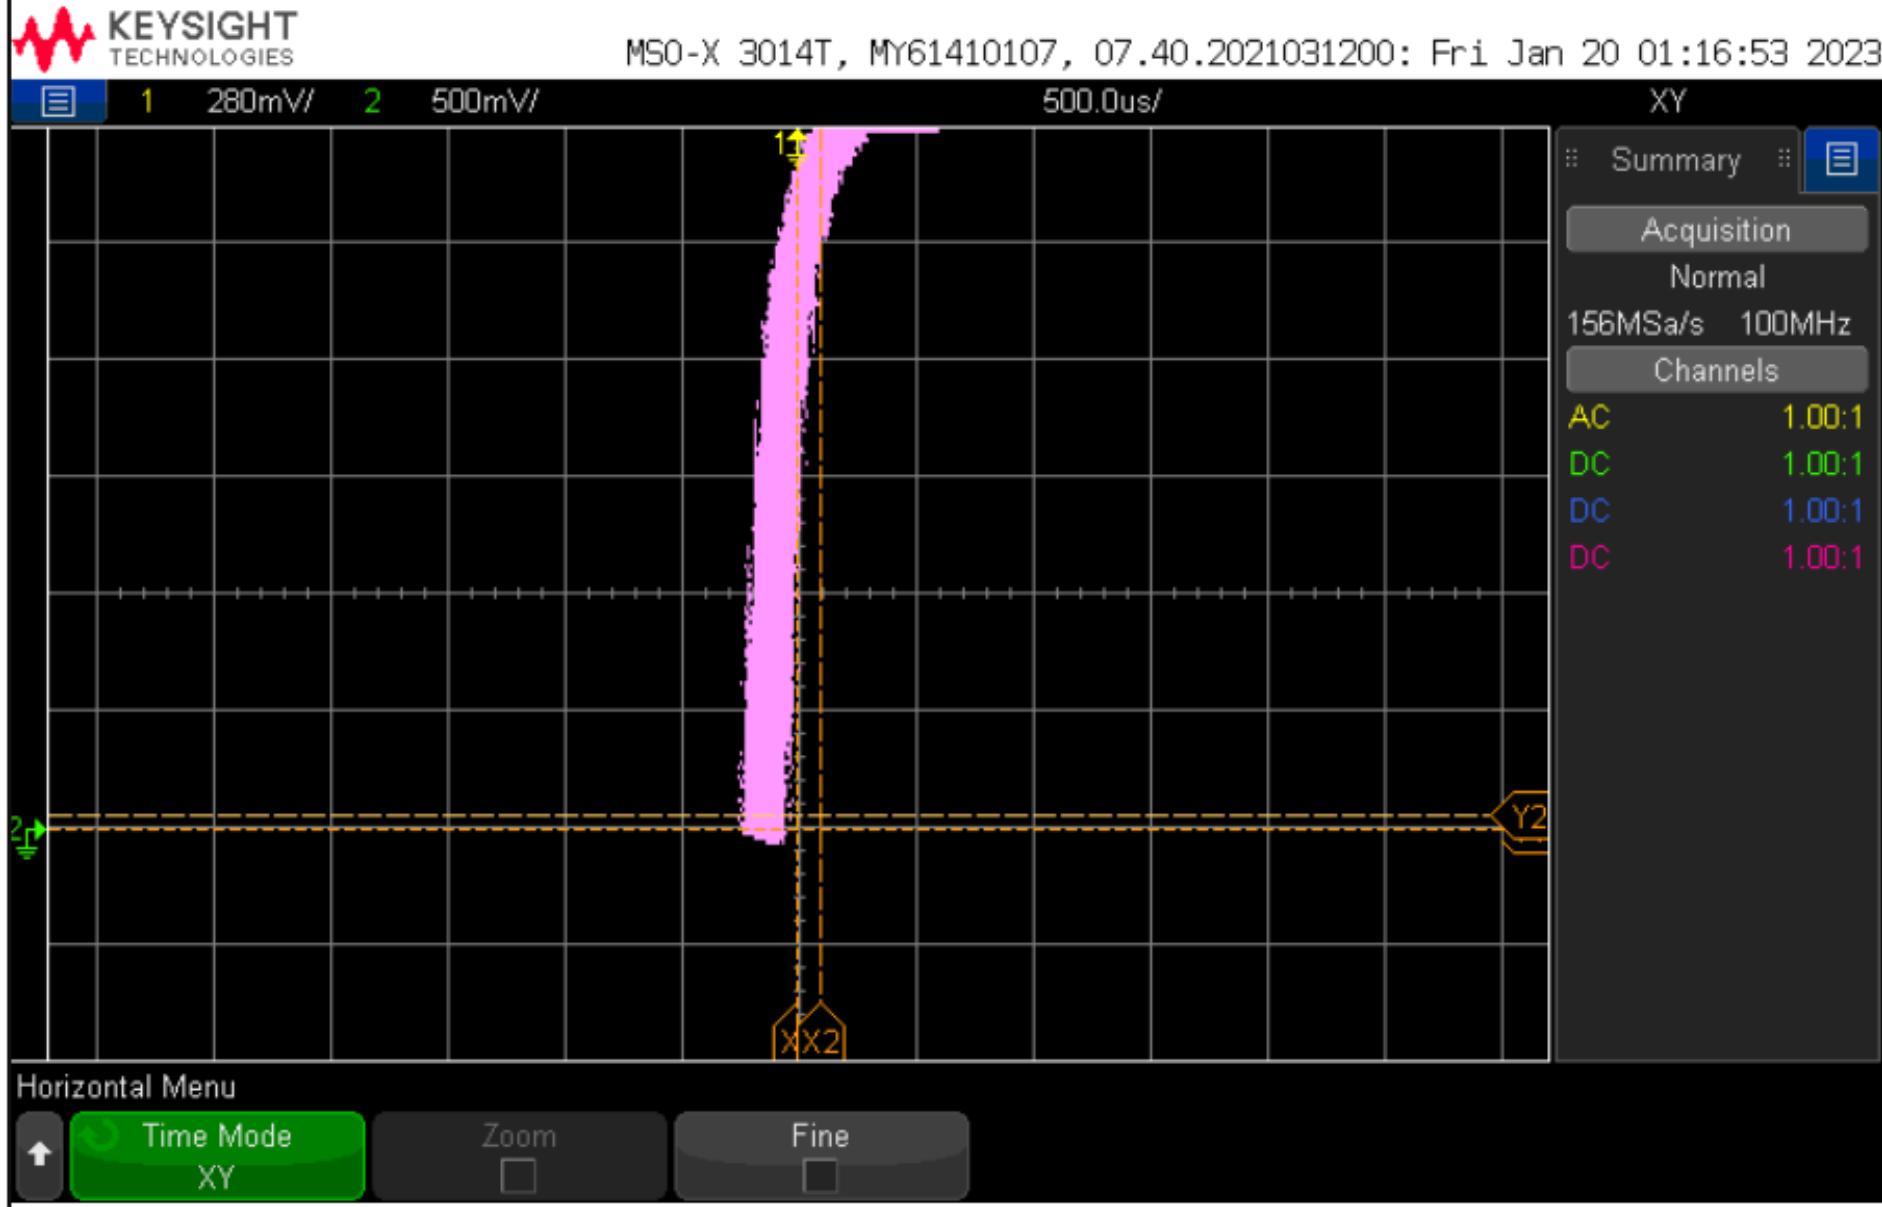
\includegraphics[scale=0.2]{linear.png}
\end{center}

\begin{center}
$v_{GS}$ = 2.2V \\
\end{center}

\newpage

\textbf{Step 5} \\

For a transistor in cutoff, the highest $V_{DS}$ and $i_D$ values measured were 2.55 V at 0.323 mA. 
Using the power equation: 

\begin{equation}
    P_{MOSFET} = V_{DS} * i_D
\end{equation}

the power in this mode can be calculated to be 0.824 mW. \\

For the first saturation plot, the highest $V_{DS}$ and $i_D$ values were 2.19 V at 8.852 mA. 
The power in this mode can be calculated to be 19.386 mW. \\

For the second saturation plot, the highest $V_{DS}$ and $i_D$ values were 1.64 V at 16.475 mA. 
The power in this mode can be calculated to be 27.019 mW. \\

For the linear region plot, the highest $V_{DS}$ and $i_D$ values were 0.35 V at 26.475 mA. 
The power in this mode can be calculated to be 9.266 mW. \\

It can be seen easily that the transistor consumes the most power when in saturation mode, and the least when in 
the linear mode. \\


\textbf{Step 6-7}\\
When $V_{GS}$ was set to a 5V DC value, the transistor's $V_{DS}$ was measured to be 3.5 mV, and the drain current $i_D$ 
was measured to be 29 mA. Using Ohm's Law,

\begin{equation}
    V = IR
\end{equation}

which can be rearranged to:

\begin{equation}
    R = \frac{V}{I} = R_{DS,on} = \frac{V_{DS}}{i_D} = \frac{0.0035 V}{0.029 A} \approx 0.120 \Omega
\end{equation}

The measured on resistance of the RFD3055LE transistor was 0.12 $\Omega$. The datasheet specifies an on resistance of
0.107 $\Omega$, which is a 12\% error. \\


\subsection*{Conclusions}
\indent\indent In this task, we created a test circuit for the RFD3055LE power transistor and determined power consumption,
working voltage values, and on resistance. We were successful in determining the values found, and all were within marginal error
when compared with the part's datasheet. \\

\newpage

\section*{Task 2}

\subsection*{Objective}
\indent\indent The objective of this task is to make a PWM motor driver circuit using the RFD3055LE power transistor.

\subsection*{Procedure}
\indent\indent \textbf{Step 1}\\
The circuit below was constructed:

\begin{center}
    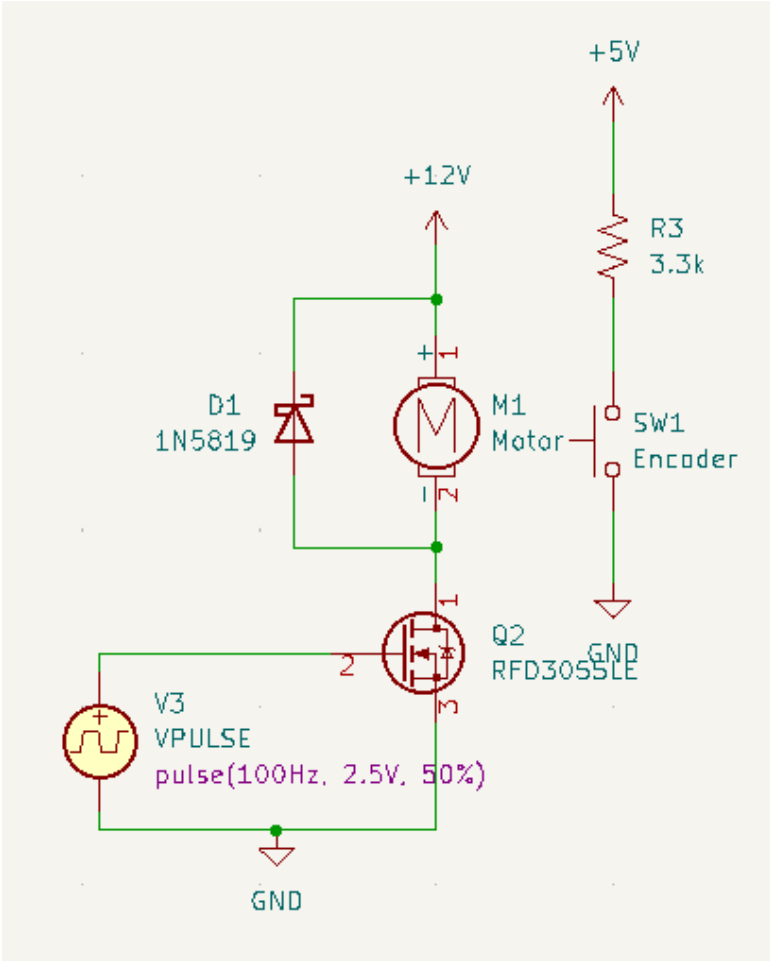
\includegraphics[scale=0.2]{task2.png}
\end{center}    

using the 1N5819 diode, and a 12V motor for the motor and encoder.\\

\textbf{Step 2-3}\\
With $v_{PWM}$ being a 0-5V 100 Hz square wave with a 50\% duty cycle, an oscilloscope screenshot was captured
showing $v_{PWM}$ and $v_{ENC}$. \\

\textbf{Step 4-6}\\
In 10\% increments, we increased the duty cycle of $v_{PWM}$ from 10\% to 90\%, while recording the motor RPM, encoder
frequency, the average drain current $i_D$ as reported by the DC power supply, and the total power consumed. The table
was then plotted on an axis of duty cycle vs. motor RPM.\\

\newpage

\subsection*{Results / Calculations}
\indent\indent \textbf{Step 3}\\
Below is a plot of $v_{PWM}$ and $v_{ENC}$ with the specifications described in \textbf{Procedure}. 

\begin{center}
    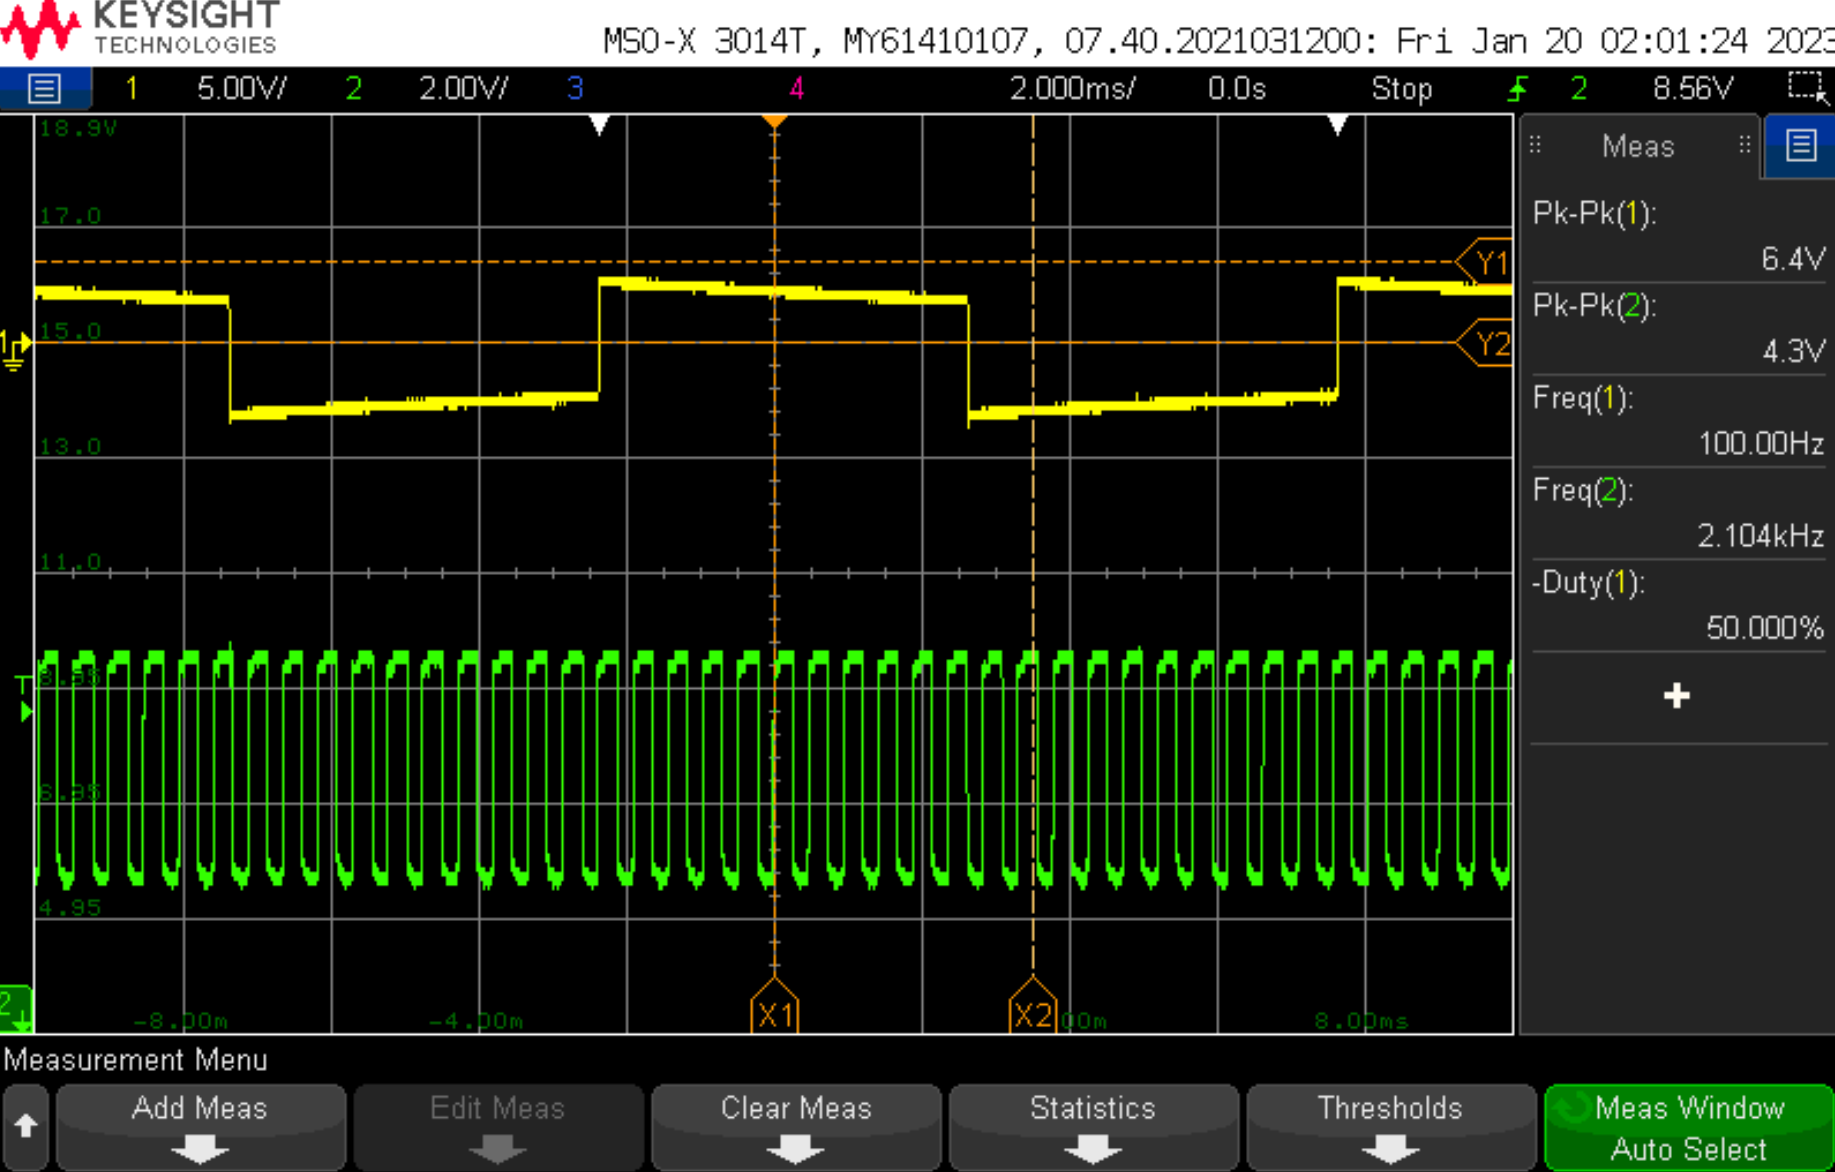
\includegraphics[scale=0.2]{t2s3.png}
\end{center}

\textbf{Step 4-5}

The following table contains the data specified in \textbf{Procedure}. The motor RPM was calculated with a simple gear reduction formula resulting 
in a ratio (Motor RPM : Encoder Frequency) being (1 : 6.233). 


\begin{table}[h!]
    \begin{center}
    \begin{tabular}{c|c|c|c|c}
    Duty Cycle (\%) & Drain Current (mA) & Encoder Frequency (kHz) & Motor RPM & Power Consumed (W) \\ \hline
    10              & 80                 & 1.26                    & 202.13    & 0.96               \\
    20              & 100                & 1.79                    & 287.16    & 1.2                \\
    30              & 112                & 1.98                    & 317.64    & 1.344              \\
    40              & 120                & 2.1                     & 336.89    & 1.44               \\
    50              & 120                & 2.13                    & 341.71    & 1.44               \\
    60              & 1.25               & 2.18                    & 349.73    & 1.5                \\
    70              & 125                & 2.2                     & 352.94    & 1.5                \\
    80              & 120                & 2.24                    & 359.35    & 1.44               \\
    90              & 118                & 2.25                    & 360.96    & 1.42              
    \end{tabular}
    \end{center}
\end{table}

\newpage

\textbf{Step 6}\\

The following is a plot of motor RPM vs. duty cycle. \\

\begin{center}
    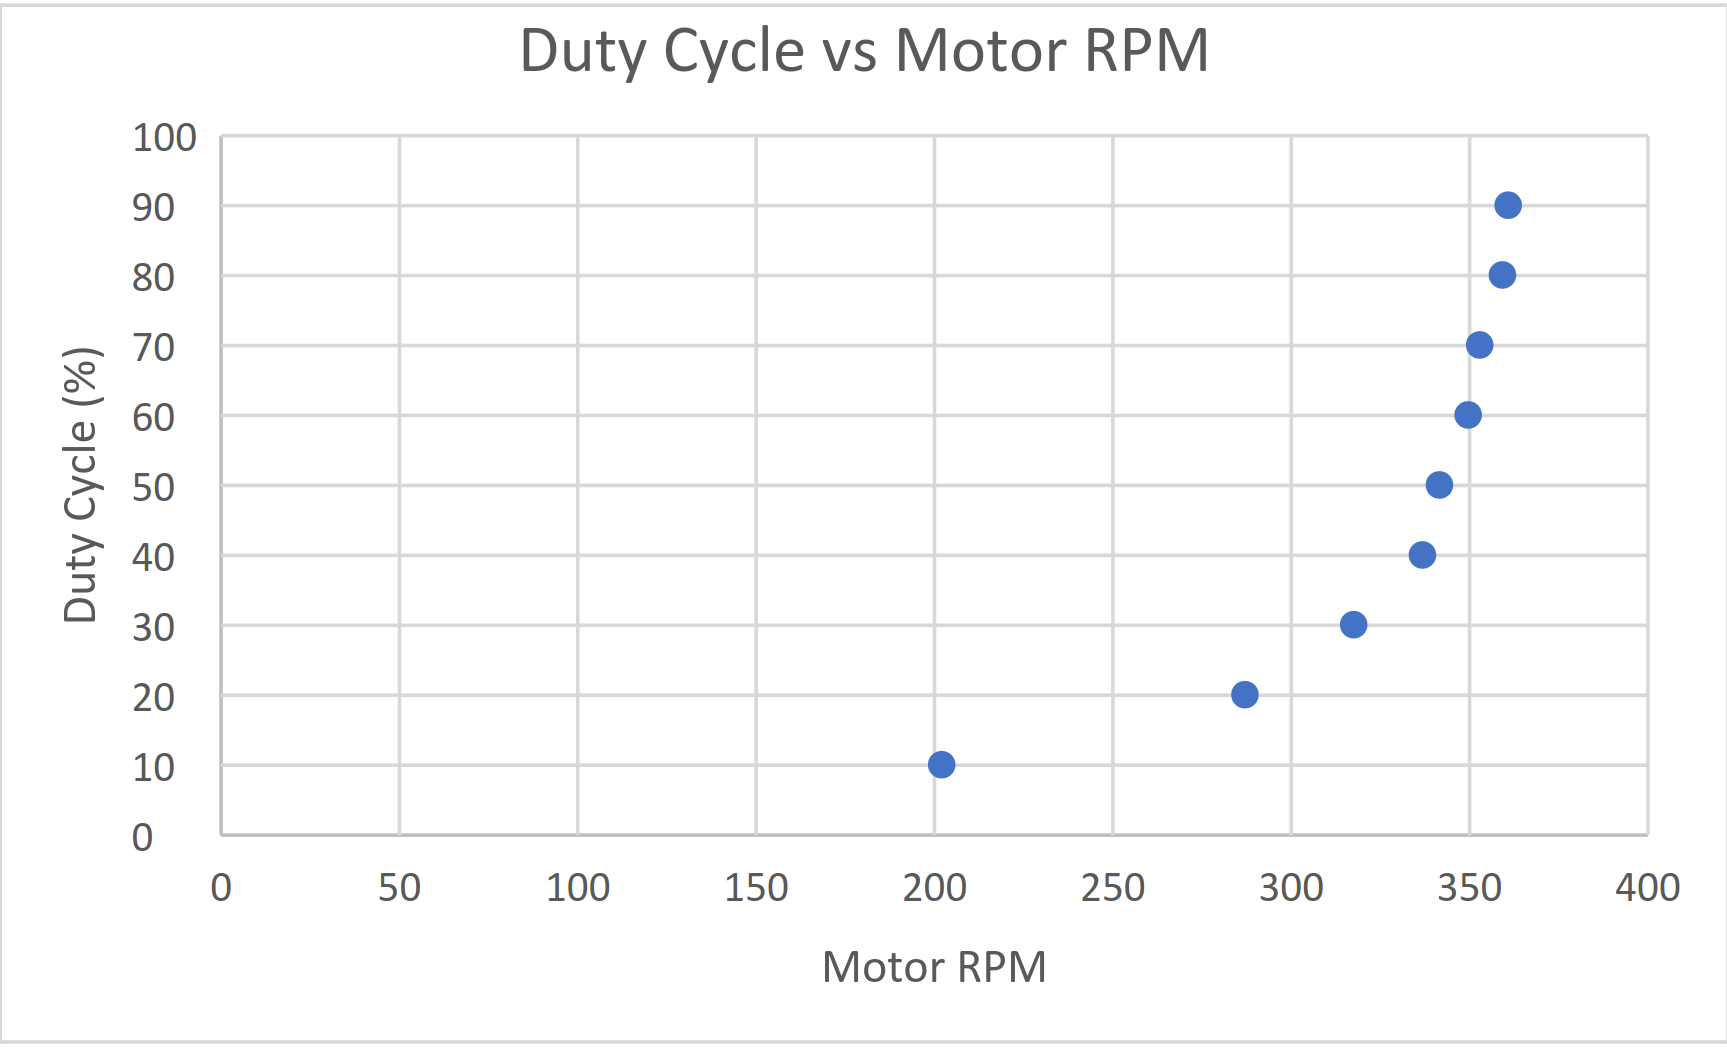
\includegraphics[scale=0.2]{plot.png}
\end{center}

The relationship between motor RPM and duty cycle is that of an exponential function. The motor RPM has a limit, which is the RPM at 
100\% duty cycle, or a flat DC value. As the duty cycle aproaches this, the motor RPM doesn't change very much. \\

\subsection*{Conclusions}

\indent\indent In this task, we created a motor driver circuit with PWM control and encoder measurement output. 
We demonstrated the motor's capability to produce different speeds at various duty cycle values, and described the relationship between the two.\\

\newpage

\section*{Task 3}

\subsection*{Objective}
\indent\indent The objective of this task is to improve upon \textbf{Task 2} by implementing a 555 timer circuit
instead of a dedicated PWM waveform input. \\

\subsection*{Procedure}

\indent\indent \textbf{Step 1}\\

The circuit below was constructed:

\begin{center}
    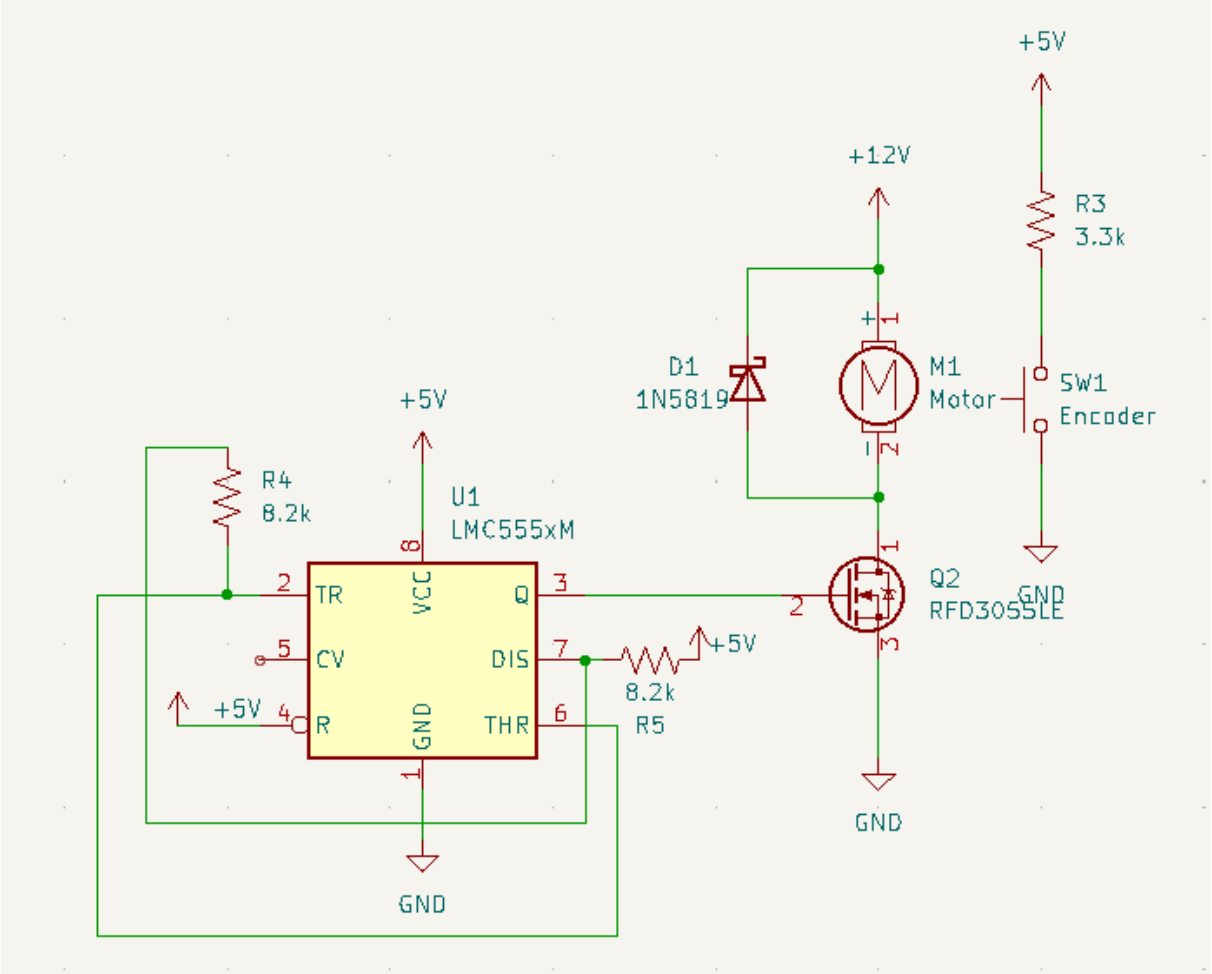
\includegraphics[scale=0.2]{task3.png}
\end{center}


\textbf{Step 2-5}\\

$V_{CTRL}$ was connected to a function generator outputting DC voltage. An oscilloscope was set up to measure $V_{PWM}$ and $V_{ENC}$. 
$V_{CTRL}$ was swept from 0V to 5V in 0.5V increments, and the duty cycle of $V_{PWM}$ was recorded, along with the motor RPM at each step.\\

Using this data, a model was created to describe the relationship between $V_{CTRL}$ and the motor speed. \\

\textbf{Step 6}\\
The function generator was replaced with a potentiometer circuit which allowed $V_{CTRL}$ to be swept from 0V to 5V using the range 
of the potentiometer. 

\newpage

\subsection*{Results / Calculations}

\indent\indent \textbf{Step 5}

The following is a table containing the data recorded when measuring motor speed and duty cycle while 
varying $V_{CTRL}$ with the function generator.\\


\begin{table}[h!]
    \begin{center}
    \begin{tabular}{c|c|c}
    Control Voltage (V) & Duty Cycle (\%) & Motor Speed (RPM) \\ \hline
    0                   & 99.6            & 0.16              \\
    0.5                 & 53              & 0.80              \\
    1                   & 12.4            & 111.97            \\
    1.5                 & 18.3            & 150.48            \\
    2                   & 25.6            & 189.63            \\
    2.5                 & 27.0            & 229.57            \\
    3                   & 41.1            & 278.34            \\
    3.5                 & 43.2            & 299.67            \\
    4                   & 48.7            & 310.75            \\
    4.5                 & 54.4            & 324.85            \\
    5                   & 60.1            & 329.36           
    \end{tabular}
    \end{center}
\end{table}

When plotted as motor speed vs. control voltage, the plot represents an exponential model, with motor speed flattening out as $V_{CTRL}$ grows.
The plot created from the table is shown below. \\

\begin{center}
    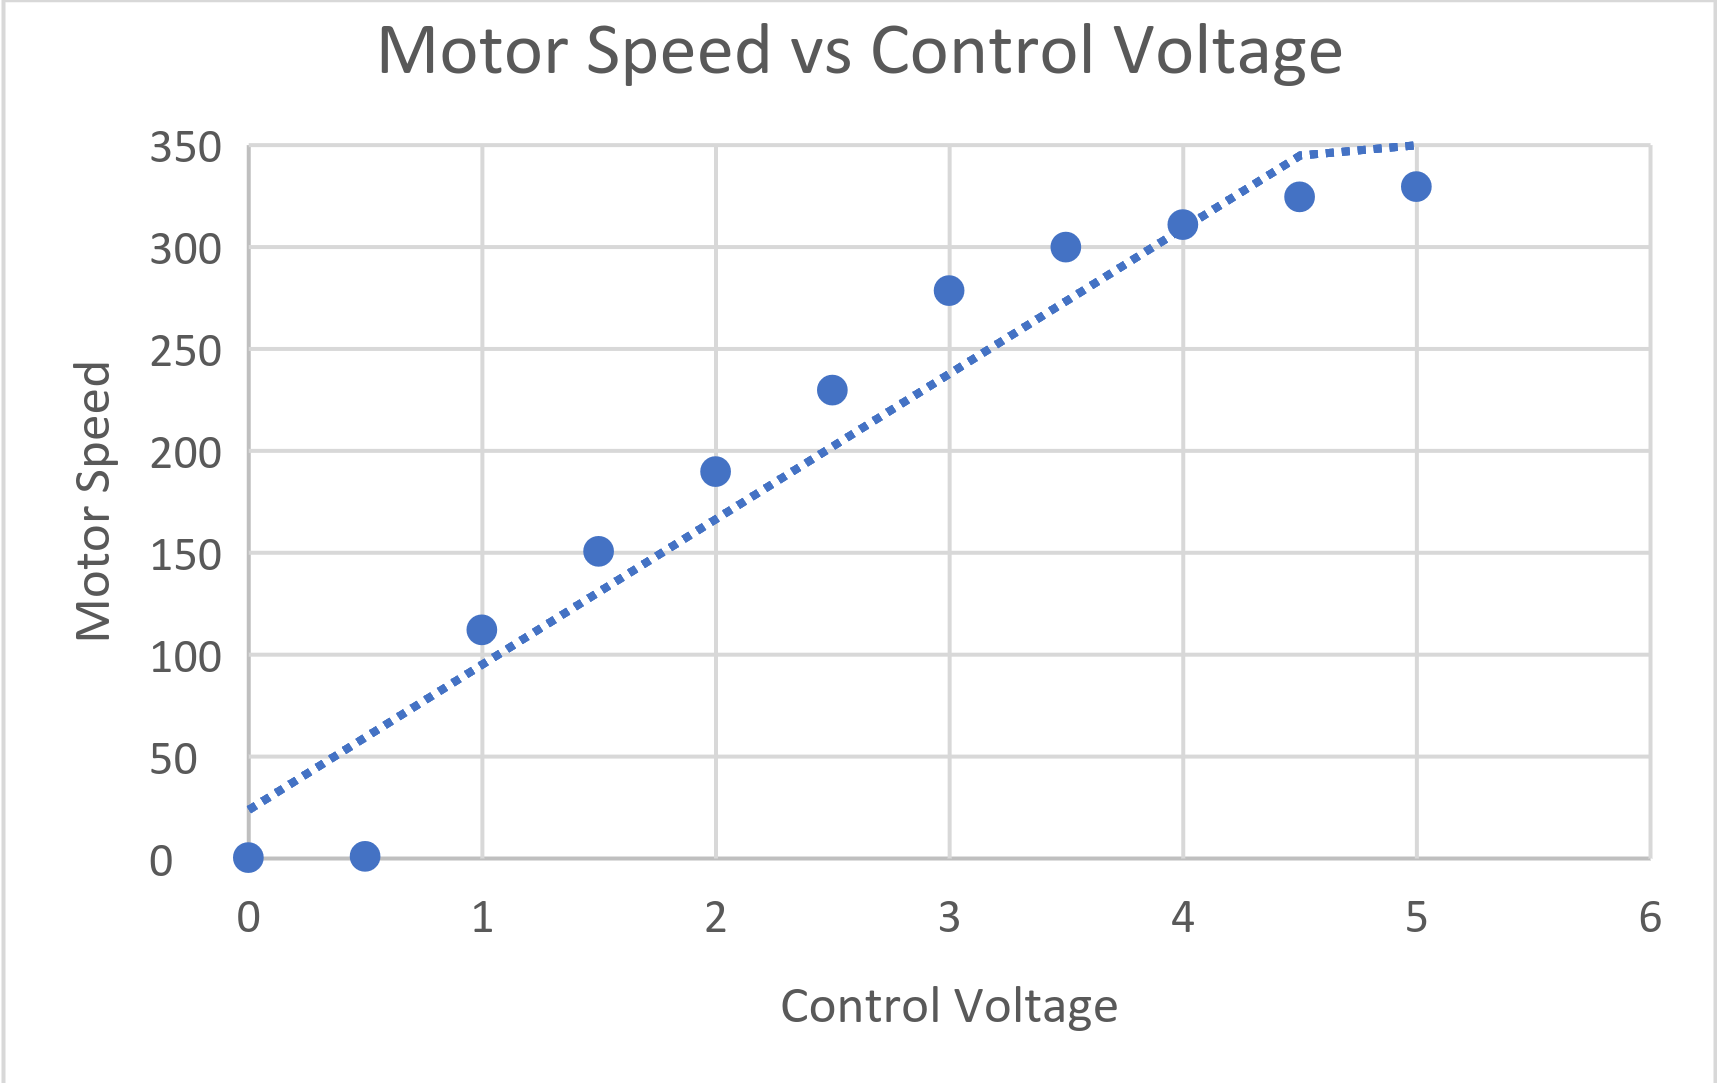
\includegraphics[scale=0.2]{graph.png}
\end{center}

\subsection*{Conclusions}
\indent\indent We were sucessful in creating a 555 timer circuit with variable duty cycle using a potentimeter. The motor's 
speed varied with maximums and minimums consistent with that which was expected. Our collected data and model also are consistent
with data gathered earlier in the experiment.\\

\newpage

\printbibliography[title={\Large References}] %Prints out the bibliography sources that you have used in the document.

\end{document}